\chapter{面向多中心用户的流行度预测方法}
\label{chap:four}
\section{引言}
社交网络已经成为人们日常生活中重要的一部分。随着时间的推移和互联网技术的发展,社交网络的功能和角色也发生了很大的变化。社交网络早期的主要功能是帮助用户在线上维护社交关系。用户可以在平台中发布自身的状态,同时也可以获取到自己关注的好友的状态信息。而当下的社交网络,更多地是在扮演着媒体的角色。从内容上看,用户在社交网络发布的内容,除却自身的状态更新外,更多地涉及当下的新闻和时事。大部分传统媒体也都直接在社交网络平台中开通了账号,便于第一时间发布各类消息。从结构上看,社交网络平台中的好友或关注机制,更多地在扮演订阅的角色。用户通过关注或者好友机制,从其他用户中获取自己感兴趣的内容。随着社交网络平台的媒体功能不断发展,进一步诞生了社交媒体的概念。借助于社交网络平台的优势,信息在社交媒体中传播地更快、更广,因此也吸引了研究者的广泛关注。

社交媒体中信息的传播模式与传统媒体有着很大的区别。在以门户网站、报纸、广播电视等为代表的传统媒体中,信息的传播都是中心式结构的:媒体是主要的发布内容者,也是用户获取信息的主要渠道,而社交媒体中信息的传播则呈现出一种去中心化的结构:信息在社交媒体中主要是沿着社交网络传播的。当用户发布信息后,他的粉丝就可以选择转发他的信息。在转发过程中,部分中间用户可能会累积大量的转发,进而使得整体的传播过程呈现出一种去中心化的结构。图\ref{fig:retweetExam}展示了新浪微博中一条消息的转发示意图,图中的每一个节点代表一个用户,每条边表示了对应用户间的转发关系。从图中可以看出,在转发过程中,有多个中间用户也累积了大量的转发,消息的整体传播结构呈现出去中心化的特点。这种去中心化的传播结构,为消息的传播预测带来了极大的挑战。
\begin{figure}[!htbp]
  \centering
  \includegraphics[width=1\textwidth]{4-retweetExam}
  \caption{新浪微博中消息的传播示例图}
  \label{fig:retweetExam}
\end{figure}

现有的用于刻画传播过程的模型主要包括基于自增强泊松过程的模型\citep{shen2014modeling,gao2015modeling}和基于自激励Hawkes过程的模型\citep{bao2015modeling,zhao2015seismic},但是这两类模型在社交媒体中刻画消息的传播过程时,都存在着各自的缺陷。基于自增强泊松过程的模型将消息的传播过程形式化为一个单源传播的过程,但是这一假设并不符合社交媒体中消息去中心化的传播模式,而且该类模型在建模每次转发带来的激励作用时,只是简单地统计消息的转发数,而没有对转发激励的大小进行区分。基于自激励Hawkes过程的模型建模了每次转发带来的激励作用,但是它需要为每一次转发学习一个激励参数,使得模型的参数学习在实际应用中难以实现,需要对模型做进一步的约减,进而影响了模型的预测能力。因此,我们仍然缺乏一个有效的用于刻画去中心化传播过程的方法。

我们对消息的传播过程进行了进一步的分析和研究,结果如图\ref{fig:multiCenter}所示。从图\ref{fig:multiCenter}(A)中可以看到,
\begin{figure}[!htbp]
  \centering
  \includegraphics[width=1\textwidth]{4-multiCenter}
  \caption{示例消息的多中心建模}
  \label{fig:multiCenter}
\end{figure}
消息整体的传播过程可以拆分为几个单源传播过程的叠加。我们将这几个单源传播过程的中心称为中心用户,并将中心用户引发的转发称为子过程。我们按照传播过程中的中心用户,将图\ref{fig:multiCenter}(A)中的传播过程拆分为6个单源传播子过程。在建模每个子过程时,我们选取了Shen等人提出的基于自增强泊松过程的RPP模型。RPP模型被提出用于解决论文引用数预测问题,非常适合单源传播的场景。RPP模型对6个子过程的建模结果如图\ref{fig:multiCenter}(B)所示。从图中可以看到,RPP模型可以很好地刻画每个中心用户引发的传播子过程。最后,我们将这6个RPP模型的预测结果按照时间顺序叠加,得到的流行度变化曲线与真实的流行度变化曲线非常相近。因此,通过叠加多个子过程来实现对消息整体传播过程的预测,是一种有效的方法。

在本章中,我们提出了一种基于RPP模型叠加的方法来刻画去中心化的传播过程。我们使用RPP模型来建模每个传播子过程,再将所有的传播子过程叠加,得到整体传播过程的建模。与基于自增强泊松过程的模型相比,我们的模型能够很好地捕获传播过程去中心化的特点,同时也区分了中心用户与其他转发用户带来的激励作用的差异;与基于自激励Hawkes过程的模型相比,我们的模型只需要学习中心用户的参数,大大减少了待学习的参数个数。

\section{数据分析}
我们在新浪微博上随机抓取了200条消息的完整转发数据,包括了转发用户、转发时间以及详细的转发路径数据,用于分析微博中的去中心化传播现象。我们从中随机挑选了几条消息的转发路径图,如图\ref{fig:diffusionTree}所示。图中的每一个点表示一条消息,消息之间的有向连边表示转发关系。我们将消息转发树中的第一个节点称为源发消息,其余节点称为转发消息。图\ref{fig:exampleD}展示是典型的中心型结构,所有消息基本上都是对源发消息的直接转发;图\ref{fig:exampleB}也是中心型的传播结构,只是部分传播链会比较长,但是没有其他消息得到大量的转发;图\ref{fig:exampleA}和图\ref{fig:exampleC}则展示了典型的去中心化结构。除源发信息外,部分转发消息本身也吸引了大量的传播,从而形成了一种多中心的传播结构。这种多中心的传播结构,目前还缺乏有效的建模方法,也是本章的建模目标。
\begin{figure}[!htb]
  \centering
  \begin{subfigure}[b]{0.4\textwidth}
    \includegraphics[width=\textwidth]{4-exampleA}
    \caption{}
    \label{fig:exampleA}
  \end{subfigure}%
  \hspace{0.05\textwidth}
  \begin{subfigure}[b]{0.4\textwidth}
    \includegraphics[width=\textwidth]{4-exampleB}
    \caption{}
    \label{fig:exampleB}
  \end{subfigure}
  \begin{subfigure}[b]{0.4\textwidth}
    \includegraphics[width=\textwidth]{4-exampleC}
    \caption{}
    \label{fig:exampleC}
  \end{subfigure}%
  \hspace{0.05\textwidth}
  \begin{subfigure}[b]{0.4\textwidth}
    \includegraphics[width=\textwidth]{4-exampleD}
    \caption{}
    \label{fig:exampleD}
  \end{subfigure}
  \caption{新浪微博中消息转发树示例}
  \label{fig:diffusionTree}
\end{figure}

为了进一步衡量微博中去中心化传播现象的比例,我们抓取了新浪微博中某一天所有的源发消息,以及这些源发消息在发布后24小时内的转发数据作为我们的实验数据。为了保证后续实验的效果,我们对数据进行了进一步的过滤。我们过滤了在发布1小时后累计转发数小于10的消息。最终我们的数据集中包含了近6.5万条源发消息以及它们的转发数据。

我们首先对源发消息的转发数据进行了统计。对于每一条源发消息,我们统计了它自身被直接转发的次数占总转发次数的比例,结果如图\ref{fig:rootRatioA}所示。图中横坐标是源发消息被直接转发的次数占消息最终总转发次数的比例,而纵坐标是转发比例小于等于对应横坐标比例的源发消息的累积分布。从图\ref{fig:rootRatioA}中可以看出,有接近20\%的消息的直接转发占总转发数的比例低于50\%,而接近50\%的消息的直接转发占总转发数的比例低于80\%,这说明直接将微博中的消息转发行为建模成单源传播是不合理的。为了消息低转发数消息对统计结果的影响,我们从数据集中剔除了最终转发数小于100的消息,并对剔除这些消息后得到的数据集进行统计,得到的统计结果如图\ref{fig:rootRatioB}所示。从图中可以看出,对于高转发数的消息来说,同样存在一定比例的源发消息,它们的直接转发占比比较低。
\begin{figure}[!htbp]
  \centering
  \begin{subfigure}[b]{0.5\textwidth}
    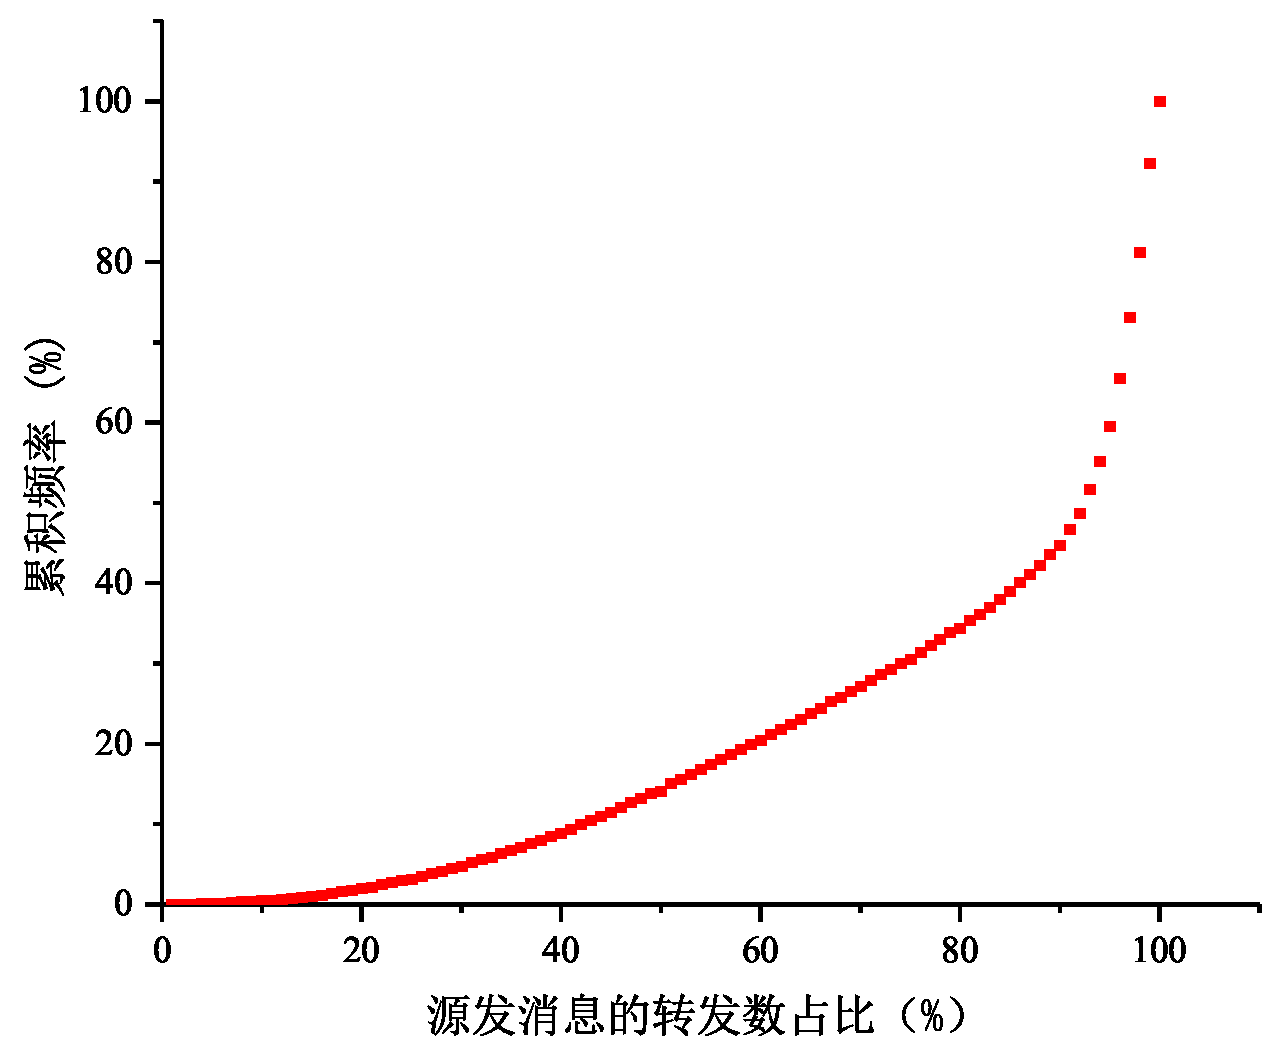
\includegraphics[width=\textwidth]{4-rootRatio}
    \caption{}
    \label{fig:rootRatioA}
  \end{subfigure}%
  \begin{subfigure}[b]{0.5\textwidth}
    \includegraphics[width=\textwidth]{4-rootRatioH}
    \caption{}
    \label{fig:rootRatioB}
  \end{subfigure}
  \caption{新浪微博中消息转发树示例}
  \label{fig:rootRatio}
\end{figure}

进一步地,我们统计了每条源发消息的转发消息引起的转发情况。对于每一条源发消息,我们搜集了它的所有的直接转发消息,统计了这些直接转发消息带来的转发数,并选取了这些直接转发消息中带来转发数最多的直接转发消息。我们统计了所选取的直接转发消息的转发数占源发消息总转发数的比例,得到的累积分布如图\ref{fig:burstRationH}所示。这里我们展示的是在剔除低转发数消息之后的数据集上的统计结果。从图中可以看出,有10\%的源发消息的直接转发消息带来的转发数占总转发数的比例超过了50\%,有20\%的源发消息的直接转发消息带来的转发数占总转发数的比例超过了30\%。这些统计结果说明,消息在传播过程中,除源发消息外还会出现少量引起大量转发的中间转发消息,对这些中间转发消息引起的转发情况的建模,是刻画去中心化传播过程的关键。
\begin{figure}[!htbp]
  \centering
  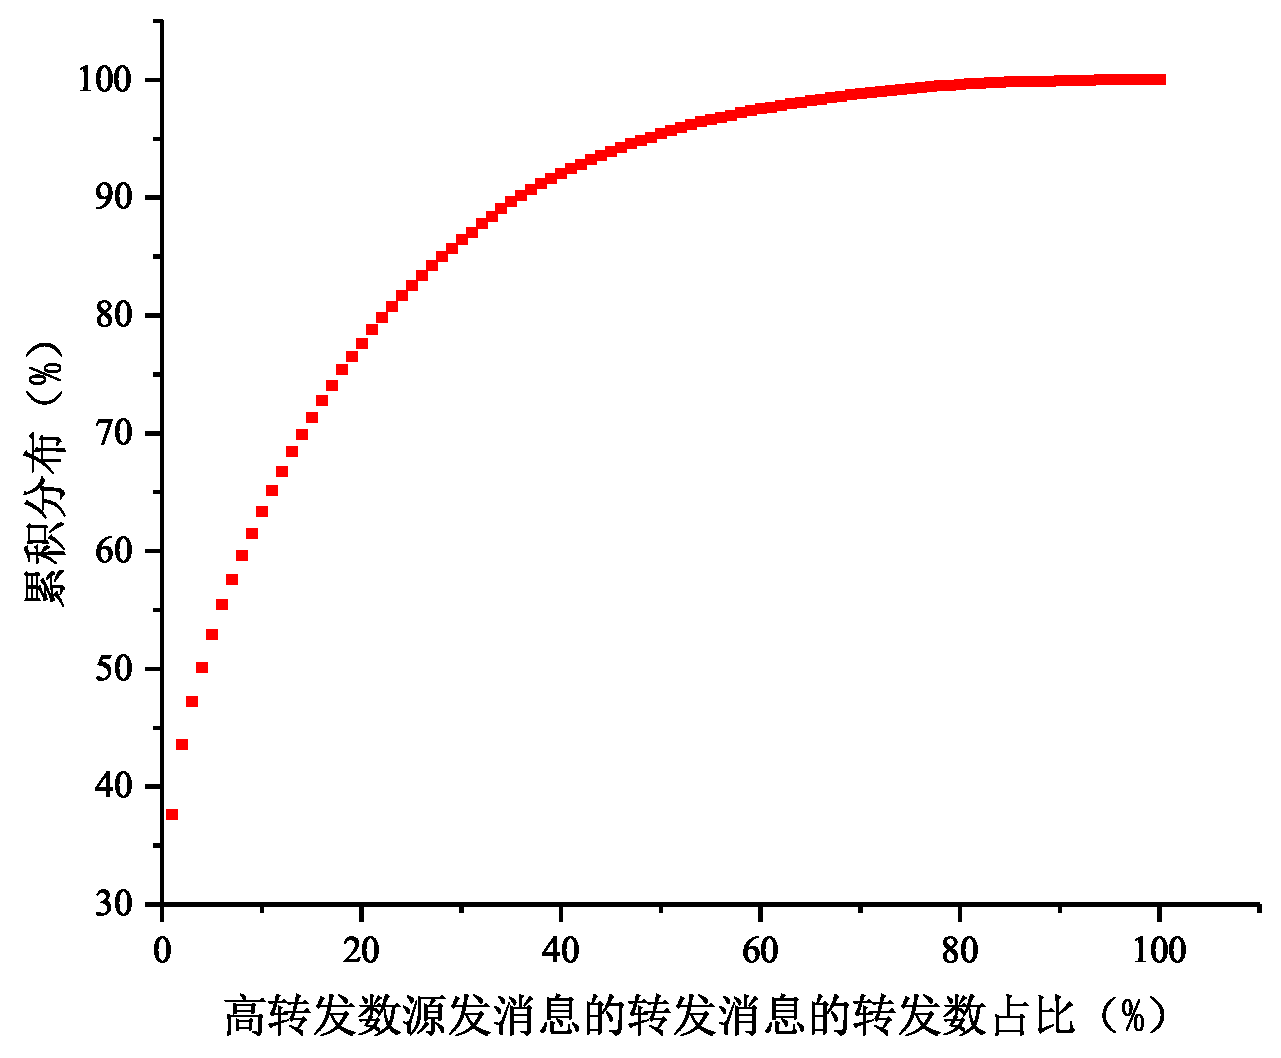
\includegraphics[width=0.5\textwidth]{4-burstRatioH}
  \caption{源发消息的转发消息引起的转发数的占比情况}
  \label{fig:burstRationH}
\end{figure}

综上所述,通过对数据集中消息的转发情况的分析,我们可以看出,去中心化的传播结构在消息传播过程中比较普遍,因此,我们需要一种模型来刻画去中心化的传播过程。进一步对各层转发消息的转发数据进行统计后发现,部分源发消息带来的直接转发数占比比较低,而部分转发消息则会带来很高的转发量。因此,刻画这些转发消息所引发的转发过程,是刻画去中心化传播过程的关键。

\section{模型}
\subsection{问题形式化}
\subsection{预备知识}
\subsection{面向多中心用户的流行度到达过程建模}
\subsection{优化}

\begin{eqnarray}
\label{eq:gradLambda}
\begin{split}
\frac{\partial lnL}{\partial \lambda_l} & = \sum_{i=1}^{n}\frac{f(t_i-t_l)}{\sum_{k=1}^{l} \lambda_k f(t_i-t_k)} + \sum_{i=1}^{n} \int_{0}^{t_i}f(t-t_l)dt - (m+n)\int_{0}^{T}f(t-t_l)dt
\end{split}
\end{eqnarray}

\begin{eqnarray}
\label{eq:gradMu}
\begin{split}
\frac{\partial lnL}{\partial \mu_l} & = \frac{1}{\sigma_l} \cdot \frac{ln(t_i-t_l)-\mu_l}{\sigma_l} \cdot \sum_{i=1}^{n}\frac{\lambda_l f(t_i-t_l)}{\sum_{k=1}^{l} \lambda_k f(t_i-t_k)} \\
& - \frac{1}{\sigma_l} \cdot\lambda_l \sum_{i=1}^{n} \phi(\frac{ln(t_i-t_l)-\mu_l}{\sigma_l}) \\
& + \frac{1}{\sigma_l}\cdot (m+n)\lambda_l \phi(\frac{ln(T-t_l)-\mu_l}{\sigma_l})
\end{split}
\end{eqnarray}

\begin{eqnarray}
\label{eq:gradSigma}
\begin{split}
\frac{\partial lnL}{\partial \sigma_l} & = \frac{1}{\sigma_l} \cdot \sum_{i=1}^{n}\{\frac{\lambda_l f(t_i-t_l)}{\sum_{k=1}^{l} \lambda_k f(t_i-t_k)}[(\frac{ln(t_i-t_l)-\mu_l}{\sigma_l})^2-1]\} \\
& -\frac{1}{\sigma_l} \cdot \lambda_l\sum_{i=1}^{n}\{\phi(\frac{ln(t_i-t_l)-\mu_l}{\sigma_l}) \cdot \frac{ln(t_i-t_l)-\mu_l}{\sigma_l}\} \\
& + \frac{1}{\sigma_l} \cdot (m+n)\lambda_l \phi(\frac{ln(T-t_l)-\mu_l}{\sigma_l}) \cdot \frac{ln(T-t_l)-\mu_l}{\sigma_l}
\end{split}
\end{eqnarray}

\begin{eqnarray}
\label{eq:gradT}
\begin{split}
\frac{\partial lnL}{\partial t_l} &= \frac{1}{t_i-t_l} \cdot \sum_{i=1}^{n}\{ \frac{\lambda_l f(t_i-t_l)}{\sum_{k=1}^l\lambda_kf(t_i-t_k)}(1+\frac{ln(t_i-t_l)-\mu_l}{\sigma_l^2}) \} \\
& -\frac{1}{\sigma_l} \cdot \frac{1}{t_i-t_l}\cdot \lambda_l\sum_{i=1}^{n} \phi(\frac{ln(t_i-t_l)-\mu_l}{\sigma_l}) \\
& +\frac{1}{\sigma_l}\cdot \frac{1}{T-t_l}\cdot (m+n)\lambda_l\phi(\frac{ln(T-t_l)-\mu_l}{\sigma_l})
\end{split}
\end{eqnarray}